\begin{frame}
	\frametitle{Ritmo de Aprendizaje}
	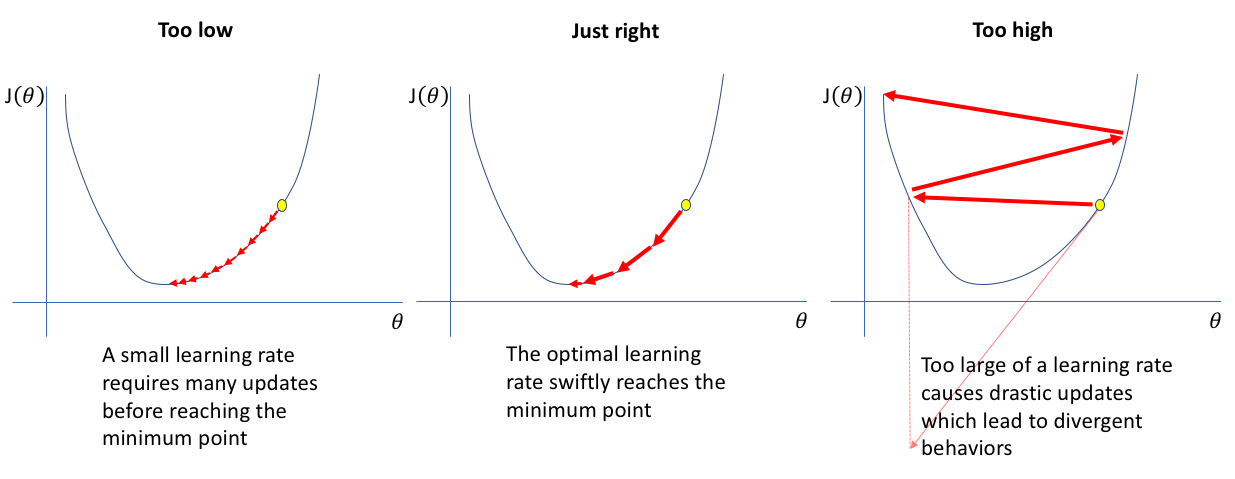
\includegraphics[scale=0.3]{learningrate}
	\begin{enumerate}
		\item ETA - El ultimo control que determina por cuanto puede cambiar el valor de un peso de una conexi\'on.
		\item Alpha - Controla el momentum con el cual estaremos ajustando los pesos de la red neuronal. 
	\end{enumerate}
\end{frame}
